Spécialiser un modèle d'intelligence artificielle implique de lui
fournir des données pertinentes, diversifiées, et en quantité
suffisante. Cependant, pour certains domaines, dont l'histoire fait
partie, le volume de données disponible est insuffisant. Ce constat est
d'autant plus vrai dans le cas des diagrammes issus de traités
astronomiques~: les corpus de documents scientifiques historiques
contiennent généralement du texte en majeure partie, des tables et des
images, négligeant souvent les diagrammes.\footnote{Exception faite du
  corpus S-VED (\cite{buttner_cordeep_2022}), collection
  d'illustration très diverses contenant entre autre des diagrammes
  historiques. Mais les primitives ne sont pas annotées.}. De plus, ils
sont dénués d'annotations précises sur les éléments constitutifs des
pages~; c'est sans parler de l'inexistence d'un corpus de diagrammes
dont les primitives sont annotées. Or l'annotation est une tâche
chronophage et fastidieuse. Le recours aux données synthétique répond,
mais en partie seulement, à ces problématiques.

\hypertarget{datasets-synthetiques}{%
\subsection{\emph{datasets} synthétiques}\label{datasets-synthetiques}}

Les \textit{datasets} synthétiques sont générés par des algorithmes ou des
méthodes de simulation pour imiter des données réelles, sans être
directement extraites de sources existantes. De tels jeux de données
sont utilisés lorsque les données réelles sont limitées ou difficiles à
obtenir, mais qu'il est cependant nécessaire de contrôler spécifiquement
les caractéristiques des données d'entraînement\footcite{buttner_cordeep_2022}. La génération
d'images a pour but de fabriquer des ensembles de données plus vastes,
plus diversifiés, très variables et assez complexes, répondant aux
caractéristiques des objets d'intérêt du projet, et surtout étiquetés
automatiquement, sans recourir à l'annotation manuelle.

Ces données synthétiques sont assez ressemblantes et complexes pour être
exploitées. Par exemple, docExtractor est un modèle off-the-shell (au
même titre que \yolo) envisagé dans le cadre de la tâche d'extraction des
diagrammes, et qui se veut sépcifique aux données historiques, car il
est entraîné sur des données produites par un générateur de documents
historiques synthétiques~: SynDoc\footcite{monnier_docextractor_2020}. SynDoc
génère des images de manière aléatoire en combinant des éléments
graphiques (fonds, images, texte et bruit) provenant d'un jeu d'image
défini (constitué de 177 images de pages, 15 contextes, plus de 8000
œuvres d'art provenant de WikiArt, des lettrines générées à partir d'une
lettre aléatoire avec 91 fonts possibles, et des dessins, schémas et
textes tirés d'articles aléatoires sur Wikipedia, avec plus de 400
fonts). Les différents éléments s'agencent, intégrant sur le fond
images, texte et bruit, offrant des combinasons et des mises en pages
assez complexes. Chaque élément de contenu est pré-annoté, éliminant
ainsi le besoin d'annotations manuelles pour ces pages.

          \begin{figure}[H]
          \begin{center}
          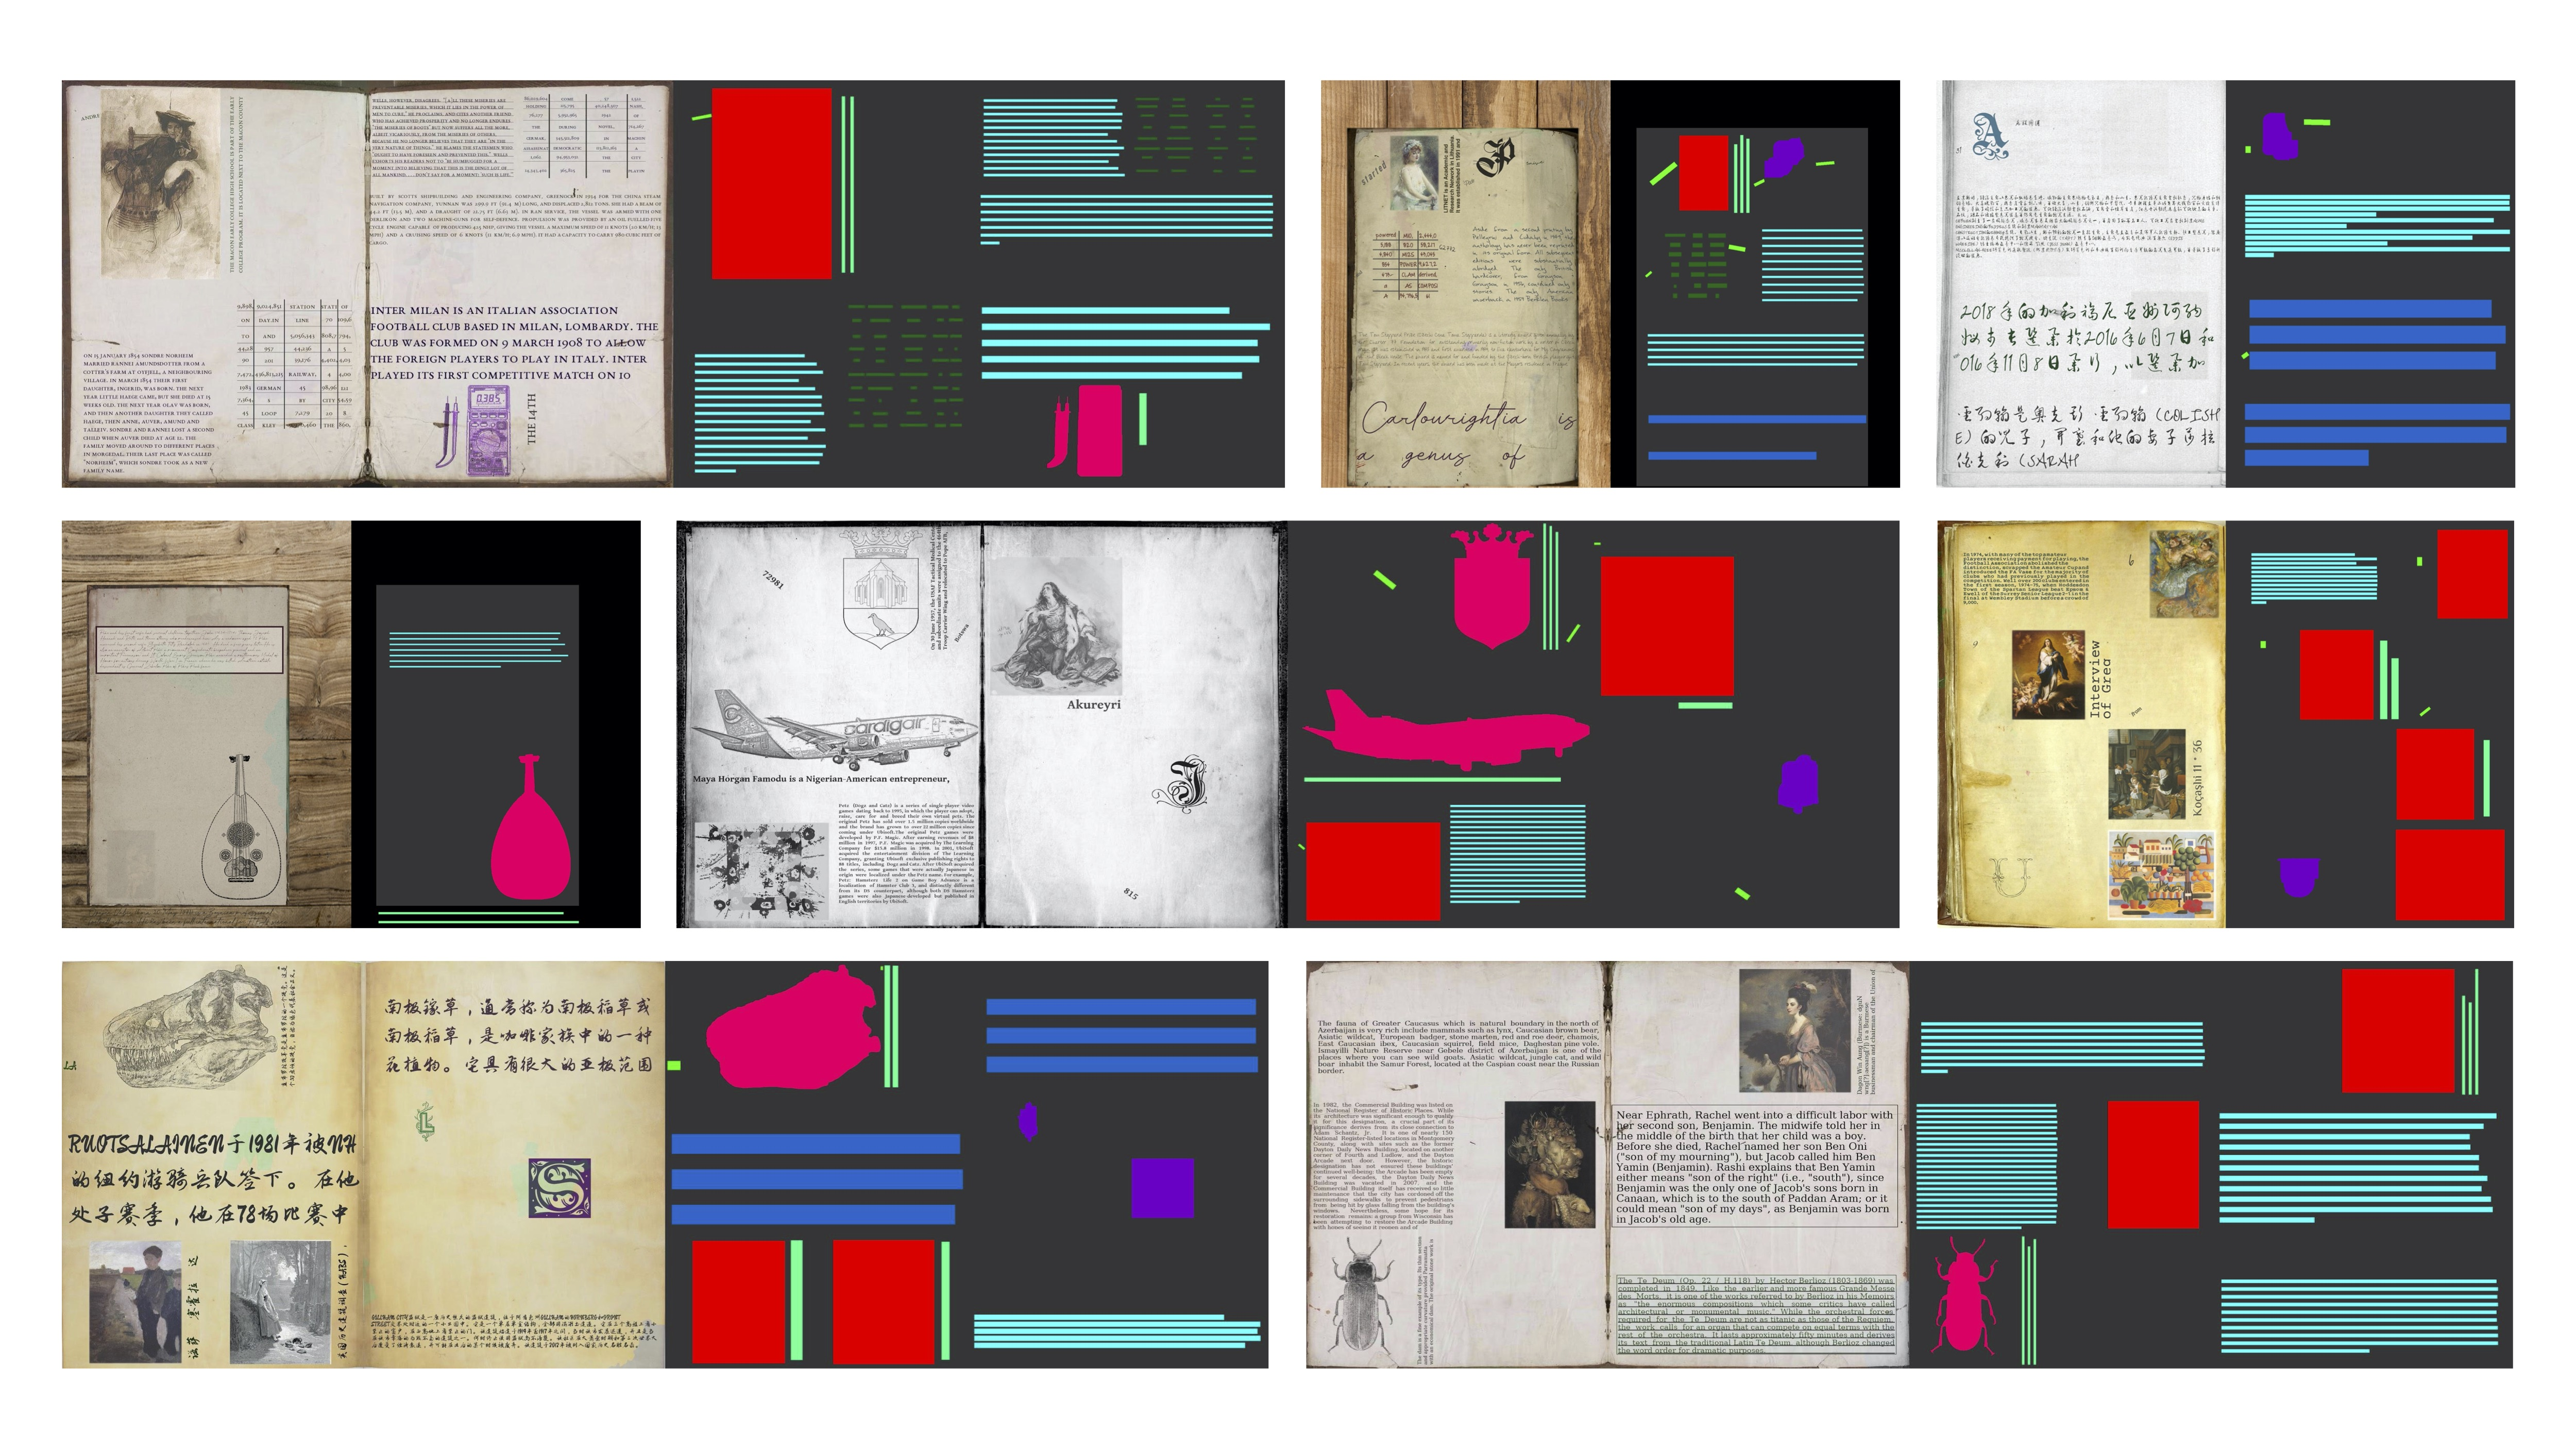
\includegraphics[height=6.5cm]{figues/syndoc.jpg}
          \end{center}
          \caption{Données synthétiques générées par SynDoc.\footcite[p.46]{norindr_traitement_2023}}
          \label{fig:syndoc} \end{figure}

Pour entraîner le modèle de vectorisation, il a de même été nécessaire
d'utiliser des données synthétiques. Parce qu'annoter les primitives
géométriques dans des images de diagrammes complexes est très
chronophage, le modèle de vectorisation a été pré-formé sur des corpus
artificiels générés dynamiquement. Le script de génération des données
d'entraînement choisit aléatoirement un arrière-plan, y ajoute des mots,
des nombres et des glyphes puis crée artificiellement un diagramme en
insérant des segments, des cercles et des arcs. Le script est conçu pour
que ces diagrammes aient une forte probabilité de présenter des formes
très caractéristiques comme les cercles concentriques et tangents, les
lignes parallèles et les arcs connectés, afin de simuler les structures
typiques. Les primitives sont dessinées avec des
variations aléatoires d'opacité, de largeur et de couleur. Les cercles
peuvent être remplis ou vides. Enfin, du bruit est ajouté en appliquant
un flou gaussien, et en supprimant de petites régions du diagramme pour
imiter la dégradation des documents historiques. Les données
d'entraînement ainsi générées présentent des configurations assez
complexes.

          \begin{figure}[H]
          \begin{center}
          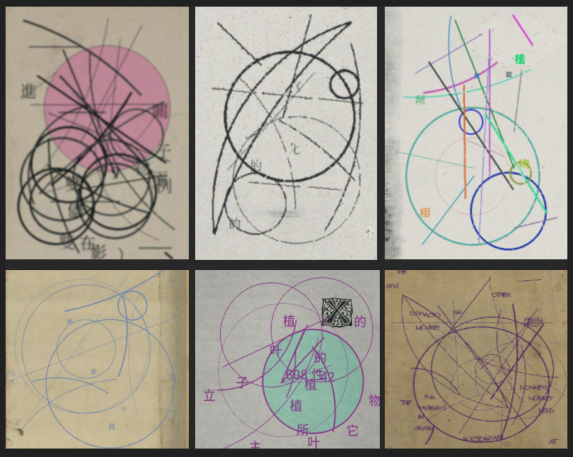
\includegraphics[height=7cm]{figues/vecto_synthetic_data.png}
          \end{center}
          \caption{Données synthétiques générées pour l'entraînement du modèle de vectorisation.\footcite[Figure issue de la présentation de Syrine Kalelli à l'occasion de la conférence \eida 2024~:][]{noauthor_eida_nodate-1}}
          \label{fig:vecto_synthetic} \end{figure}

Enfin, le modèle de similarité présente un troisième exemple, puisque
SegSwap est pré-entraîné sur de la donnée synthétique. Le script de
génération prend des parties aléatoires d'une images et les copie-colle
au-dessus d'une autre image. Les trois images (source, cible et
superposition) sont placées dans le même dataset d'entraînement, ainsi
le modèle apprend à retrouver ce qui, dans la superposition, vient de la
source, et ce qui vient de la cible.

          \begin{figure}[H]
          \begin{center}
          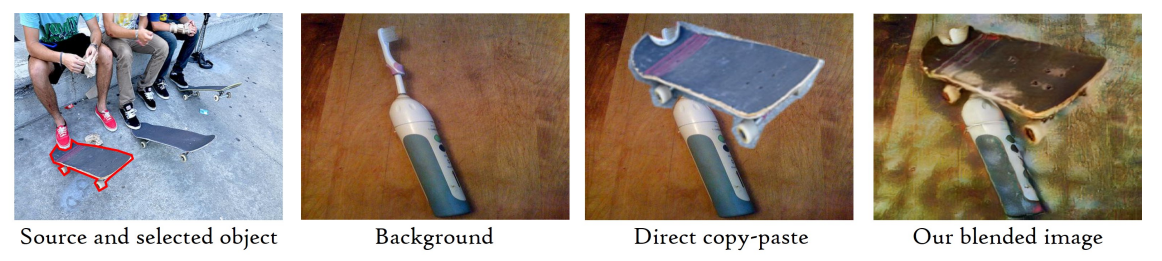
\includegraphics[height=3cm]{figues/segswap_blended_images.png}
          \end{center}
          \caption{Données d'entraînement du modèle Segswap.}
          \label{fig:segswap} \end{figure}

\hypertarget{les-donnees-reelles}{%
\subsection{Les données réelles}\label{les-donnees-reelles}}

S'appuyer sur les modèles \textit{off-the-shelf}, sur de larges \textit{datasets}
généralistes, ou sur des données synthétiques permet une implémentation
facilitée de la vision dans des projets et constitue une base solide.
Toutefois, les sources tenant aux deux projets (\vhs et \eida) sont trop
spécifiques pour se contenter de modèles généralistes ou formés sur des
données artificielles. Même si ces derniers peuvent offrir des performances
de base, ils risquent de manquer de précision et de sensibilité aux
particularités des documents historiques. Les corpus artificiels
présentent des configurations délibérément complexes pour s'approcher le
plus possible des difficultés que le modèle pourrrait rencontrer sur les
données réelle. Elles sont cependant irréalistes et insuffisantes pour
permettre aux modèles de généraliser sur des diagrammes réels.

En atteste la comparaison des performances de docExtractor et \yolov sur
les données d'\eida. docExtractor\footcite{monnier_docextractor_2020}, entraîné
sur des données synthétiques mimant les documents historiques serait en
théorie plus adapté au traitement d'images de pages de manuscrits, avec
du texte et des illustration côté à côte, d'autant qu'il intègre des
outils de traitement du texte (notamment pour la segmentation des
lignes)\footnote{\eida envisage l'implémentation d'un outil d'extraction
  et transcription des labels et des textes qui entourent les diagrammes}.
Pourtant, sans fine-tuning sur des données réelles, il présente des
performances équivalentes à celles de \yolov\footcite[p.45]{norindr_traitement_2023}. Cela
souligne que même les modèles off-the-shelf entraînés sur un corpus
assez spécifique et complexe, mais synthétique, ne dispense pas d'un
entraînement sur des données réelles, au même titre que les modèles très
généralistes comme \yolov.

Alors, le modèle de base \yolov tel que mis à disposition par
Ultralytics est entraîné sur de grands ensembles de données réelles, ce
qui constitue une base solide pour la classification des objets du
monde. L'utilisation de SynDoc permet ensuite de compléter
l'apprentissage initial en exposant le modèle à des exemples variés et
spécifiques aux documents historiques, augmentant ainsi sa capacité de
généralisation. Ces similis de manuscrits anciens offrent l'avantage de
pouvoir être produits en grandes quantités et de couvrir un large
éventail de scénarii et de configurations difficiles à obtenir dans des
ensembles de données réelles. Puis le modèle est entraîné sur les
données de \vhs, qui sont de réelles pages de documents historiques
contenant une large diversité d'illustrations. Ces données apporteront
une dimension supplémentaire de pertinence au modèle, en l'exposant à
des particularités des documents historiques réalistes. Enfin, \yolov
est entraîné sur les données d'\eida, qui sont orientées spécifiquement
vers les diagrammes, afin qu'il détecte uniquement ces derniers.

Quant au modèle de vectorisation développé par Syrine
Kalleli\footcite{kalleli_historical_2024}, il est formé
sur des données synthétiques générées à la volée par un script. Mais le
corpus de diagrammes d'\eida est particulièrement caractéristique et le
modèle n'aurait pu être optimal sans avoir appris sur des images de
diagrammes issus de manuscrits réels. Un corpus d'entraînement de 303
diagrammes extraits de manuscrits et de gravures a donc été constitué et
annoté par les historien.nes. Ces diagrammes sont issus de sources latines, arabes,
grecques, hébreuses ou chinoises, datant du \textsc{xii}\ieme au \textsc{xviii}\ieme siècle, et ils
présentent en guise d'étiquettes plus de 3000 lignes, cercles et arcs. Le
ré-entraînement a permis le transfert des connaissances acquises sur la
tâche de détection des primitives sur les données réalistes.

Il sera également possible d'obtenir des meilleurs résultats sur la
similarité grâce à une évaluation des scores (qui constitue un jeu de
données annotées) et le ré-entraînement du modèle, pour donner des
résultats plus adaptés à la spécificité des données historiques.

D'ailleurs, cette étape d'annotation (le choix des exemples et des
étiquettes) revêt des enjeux importants. L'apprentissage spécifique se
fait à partir de données sélectionnées par les chercheur.ses~: les exemples
sur lequel l'algorithme d'apprentissage va itérer définissent le modèle.
Il est nécessaire de constituer un échantillon de données aléatoire et
représentatif, et de l'annoter en fonction de ce que l'on souhaite
obtenir en prédiction.

L'annotation des jeux de données est non seulement une étape clé, mais
aussi un bel exemple de collaboration chercheur.ses-ingénieur.es. Elle
nécessite la définition de normes pertinentes et rigoureuses. Travail
minutieux et chronophage, l'étiquetage des données peut engendrer des
erreurs et du bruit dans les données, car elle implique la subjectivité
des chercheur.ses et le regard parfois trop précis sur les sources desquels
les annotateurs sont experts.

Voici un exemple rencontré lors de la préparation des données pour
entraîner un modèle de segmentation du contenu textuel. Les sources
arabes et chinoises sont particulièrement verbeuses et les diagrammes
sont très souvent entourés des blocs de commentaires se mélangeant alors
aux légendes et aux labels. Doit-on considérer ces commentaires comme
faisant partie des éléments que l'on souhaite identifier ou bien les ignorer
? Cette décision est importante car si on les ignore, le modèle risque
de passer à côté d'éléments textuels pertinents. En revanche, si on les
inclut, il ramènera des commentaires sans rapport direct avec le
diagramme observé. On voit ici comment la binarité des modèles, qui se
reflète dans les normes d'annotation, est problématique et constitue une
limite au \ml. Un compromis doit être trouvé entre
l'automatisation, qui requiert une normalisation, des définitions
claires et binaires, et la nuance dans l'interprétation des
sources\footnote{Dans le cadre du projet, il a toujors été plus
  intéressant d'opter pour une définition extensive des objets à
  détecter, car prévision d'une correction des traitement. Et il est
  plus facile de supprimer un élémént pas pertinent que d'aller en
  rechercher un, surtout compte tenu de la taille des corpus des
  chercheur.ses. Vaut aussi pour la préparation des données pour
  l'entraînement du modèle d'extraction.}.

La normalisation peut bénéficier à l'écosystème de recherche dans le
domaine de l'\htr et de l'\ocr. À ce titre, il est pertinent d'envisager
l'utilisation du vocabulaire contrôlé SegmOnto pour l'annotation du
contenu textuel entourant les diagrammes. Cela permettrait de créer des
jeux de données réutilisables, à partager avec des projets poursuivant
des objectifs similaires.\footnote{https://segmonto.github.io/}. Encore
une fois, un compromis doit être trouvé entre les besoins de description
des chercheur.ses et les possibilités offertes par les vocabulaires
contrôlés.

Un autre exemple concerne le dernier entraînement du modèle d'extraction
: les résultats montrent que des diagrammes sont encore détectés en
transparence. La question s'est alors posée de chercher à corriger ce
défaut en donnant au modèle, à l'occasion d'un nouvel entraînement,
d'avantage d'exemples négatifs (diagrammes visibles par transparence
mais non annotés). Or il est préférable de se contenter de la correction
ou suppression manuelle de ces prévisions erronées, garantissant que le
modèle parvienne à détecter les diagrammes presque effacés.

Pour assurer la rigueur et la cohérence des annotations, les décisions
prises entre les chercheur.ses et les ingénieur.es peuvent être l'objet d'une
documentation ou d'ateliers d'annotation.

\hypertarget{loeil-de-la-machine-avantages-et-limites}{%
\subsection{L'oeil de la machine~: avantages et
limites}\label{loeil-de-la-machine-avantages-et-limites}}

Bien qu'il soit possible d'optimiser les performances d'un modèle
d'apprentissage automatique en l'entraînant sur un ensemble de données
spécifique, son interprétation des données reste limitée car
fondamentalement binaire, ce qui le rend parfois déficient pour la
recherche en histoire. Ainsi, il gèrera difficilement les cas limites et
ambigüs. La décision d'inclure ou d'exclure ces cas particuliers de
l'ensemble d'entraînement implique un arbitrage délicat. D'un côté, une
inclusion trop restrictive peut compromettre les capacités de
généralisation du modèle, c'est-à-dire sa capacité à s'adapter à de
nouvelles données. À l'inverse, une inclusion trop permissive risque de
dégrader la précision du modèle sur les cas plus typiques. Les
chercheur.ses espérant obtenir un modèle maximaliste, quitte à accepter un
certain degré d'erreur et de devoir supprimer les faux
positifs, de nombreux cas limites ont été inclus. Le cas des diagrammes
visibles en transparence (expliqué précédemment) en est un exemple
éloquent.

Une autre difficulté réside dans la définition même du ``diagramme
astronomique''. Les limites de ce concept ne sont pas si claires et
définitives pour les chercheur.ses, et pourtant le modèle a besoin d'une
définition rigoureuse et cohérente. Il paraît en effet difficile de
considérer les diagrammes astronomiques en dehors du contexte des
pratiques d'autres sciences et disciplines connexes. Par exemple, Le
\emph{Flores Almagesti} -- réécriture de l'Almageste datant du \textsc{xv}\ieme par
l'astronome Giovanni Bianchini -- présente une partie algébrique à
l'ouverture mathématique, induisant la présence de nouveaux types de
diagrammes d'inspiration euclidienne. Pour retracer la source de ces
derniers, il est nécessaire de considérer les traités d'Euclide ou
autres travaux d'algèbre. Ceux-ci ne sont pas des traités
\emph{astronomiques}, bien qu'il ne soit pas certain que ces disinctions
contemporaines aient été aussi rigide à l'époque et aient eu un
quelconque sens pour les acteurs historiques. Les sources byzantines
confirment cette complexité~: les diagrammes y sont nommés
\emph{katagraphai}, indépendamment du domaine scientifique auquel ils
appartiennent. Également, de nombreux travaux astronomiques sont groupés
dans des témoins qui contiennent des œuvres issus de domaines divers.
C'est le cas avec les sources chinoises, comme le \emph{Chongzhen
lishu}, qui se présente généralement annexé d'une série de traités
mathématiques. Par conséquent, les diagrammes euclidiens ont été gardés
lors de la préparation des données, et l'algorithme de détection les
classe comme ``diagramme'', même s'ils ne constituent pas l'objet
principal des chercheur.ses.

En ce qui concerne les autres types de diagrammes non strictement
astronomiques (géométriques, harmoniques, logiques, illustrations de
constellations), une approche plus sélective a été adopté afin d'éviter
un modèle trop maximalistes. Ces éléments, bien que potentiellement
intéressants, n'ont pas été inclus dans la phase de détection
automatique.

Ainsi l'œil de la \cv contraint à des choix méthodologique
potentiellement inconfortables, mais en même temps il peut aider à
mesurer les impulsions des chercheur.ses, à mieux définir les objectifs de
recherche et à prioriser les éléments les plus pertinents. Ainsi, la
vision par ordinateur oblige les chercheur.ses à s'adapter à une logique
algorithmique qui, tout en limitant certaines interprétations
subjectives, offre l'opportunité de développer des modèles conceptuels et des méthodologies très rigoureuses.